% (c) Gerard Baecker
\documentclass[fleqn,a4paper,12pt]{article}
\usepackage[german]{babel}
\usepackage[utf8]{inputenc}
\usepackage{amsmath}    % Mathematische Symbole
\usepackage{amssymb}     % Nochmehr mathematische Symbole
\usepackage{dsfont}      % Schriftsatz fuer Zahlenmengensymbole
%\usepackage{verbatim}   % erweiterte Verbatim-Umgebung
\usepackage{alltt}       % Quasi-Verbatim-Umgebung
\usepackage{fancyhdr}    % Eigene Kopfzeilen
\usepackage{graphicx}    % Zum Einbinden von Grafiken
% Einbinden einer eps-Grafik geht so: includegraphics{path}

% Seitenraender
\addtolength{\voffset}{-2cm}
\addtolength{\textheight}{0cm}
\addtolength{\hoffset}{0cm}
\addtolength{\textwidth}{2cm}
\addtolength{\headheight}{2cm} % fuer jeden Strichkode einen Zentimeter

% Skalierung der Grafiken
\setlength{\unitlength}{1cm}

\pagestyle{fancy}            % Eigene Kopfzeilen verwenden
\frenchspacing               % Kein Extrafreiraum nach Satzzeichen
\setlength{\parindent}{0pt}  % Neue Absaetze nicht einruecken
%\sloppy                     % Schlampige Absatzformatierung
\fussy                       % Penible Absatzformatierung
\linespread{1.5}             % Zeilenabstand

% Font fuer Code 39
\font\xlix=wlc39 scaled 1200
\newcommand\barcode[1]{{\xlix@#1@}}

% Name, Matrikelnummer, Barcode
\newcommand\student[2]{
	\mbox{\scriptsize
		\begin{tabular}{@{}l@{}r@{}}
			\multicolumn{2}{@{}r@{}}{\barcode{#2}}\\
			#1&#2\\
\end{tabular}}}

% Kopfzeile
\lhead{
	\small
	\textsc{Grundlagen der Signalverarbeitung \\
		WS 2017/2018 \\
		\"Ubung (\today)}
	\vfill}
\rhead{
	\begin{tabular}[b]{@{}rr@{}}
		\student{Philipp Badenhoop}{572693} &
		\student{Steven Lange}{789012} \\
		\student{Pascal Jochmann}{575056} &
		\student{Kevin Trogant}{572451}
\end{tabular}}

\begin{document}
Aufgabe 11)

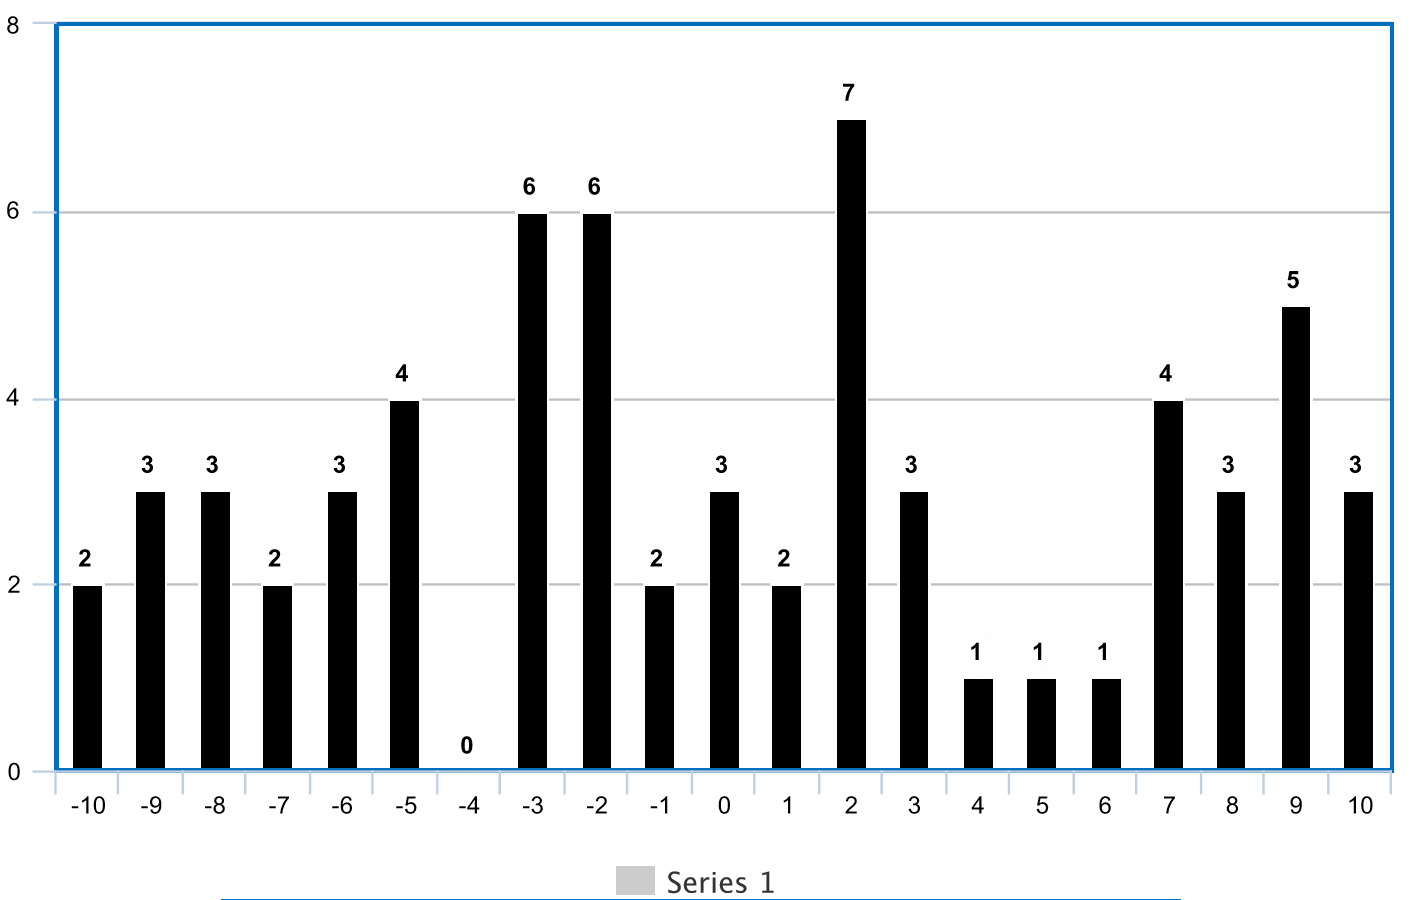
\includegraphics[scale=0.4]{H2}

a)Ganzes Signal:\\
$m_1 = 0,19		z_2 = 35$ \hspace{1cm}
Median = 0,	Modalwerte: -4 und 2

Signal in zwei H\"alften:\\
Erste H\"alfte:	\hspace{5cm}										Zweite H\"alfte:\\
$m_1 = 0,219$  $z_2 = 25$	\hspace{4cm}								$m_1 = -0,157$  $z_2 = 24$\\
\\
b)\\
Es K\"onnen 16 nicht \"uberlappende Episoden heraugeschnitten werden.
Episodemittelswertvektor: $m = \frac{1}{M}\sum_{i=0}^{M-1}e_i$\\
 $m = (-2,94, 1,38, 1,25, 1,06)^T$\\
 Keiner der Scharmittelwerte entspricht m1 $\rightarrow$ Signal ist weder station\"ar noch ergodisch.
 \newpage
 Kovarianzmatrix: $S = \frac{1}{M}\sum_{i=0}^{M-1}(e_i-m)(e_i-m)^T$\\
 $
\begin{bmatrix}
21   & -6,3 & 1,4	 &  -1,8 \\
-6,3 & 44 	& -18	 &  -8 \\
1,4  & -18	& 29 	 & -4,3 \\
-1,8 & -8 	& -4,3	 &  34
\end{bmatrix}
$\\
Korrelationsmatrix $R_{u,v} = \frac{S_{u,v}}{\sqrt{S_{u,v} \sqrt{S_{u,v}}}}$
 $
\begin{bmatrix}
1   & -0,21 & 0,06	 &  -0,07 \\
-0,21 & 1 	& -0,5	 &  -0,21 \\
0,06  & -0,5	& 1 	 & -0,14 \\
-0,07 & -0,21 	& -0,14	 &  1
\end{bmatrix}
$\\Die Werte abseits der Hauptdiagonale sind (im Betrag) klein, $\rightarrow$ das Signal ist zuf\"allig\\

\newpage

Aufgabe 12)

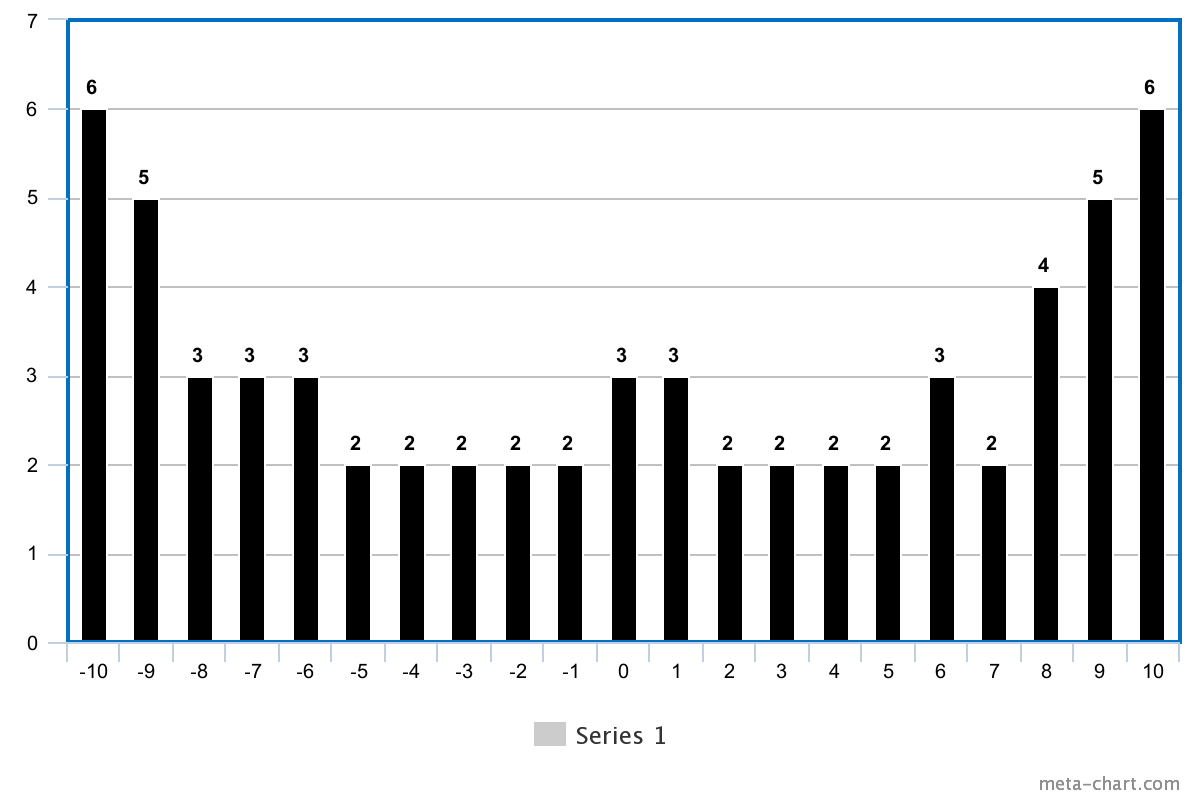
\includegraphics[scale=0.4]{H3}

a)Ganzes Signal:\\
$m_1 = 0,031		z_2 = 49$ \hspace{1cm}
Median = 0,	Modalwerte: $\pm $10

Signal in zwei H\"alften:\\
Erste H\"alfte:	\hspace{5cm}										Zweite H\"alfte:\\
$m_1 = 0,21875$  $z_2 = 25$	\hspace{4cm}								$m_1 = -0,15625$  $z_2 = 24$\\
\\
b)\\
Es K\"onnen 16 nicht \"uberlappende Episoden heraugeschnitten werden.
Episodemittelswertvektor: $m = \frac{1}{M}\sum_{i=0}^{M-1}e_i$\\
$m = (0, 0,063, 0, 0,063)^T$\\
Seine Scharmittelwerte sind \"ahnlich $m_1 \rightarrow$ Signal ist  station\"ar und ergodisch.
\newpage
Kovarianzmatrix: $S = \frac{1}{M}\sum_{i=0}^{M-1}(e_i-m)(e_i-m)^T$\\
$
\begin{bmatrix}
49   & 45 & 33	 &  16 \\
45 & 49 	& 45	 &  33 \\
33  & 45	& 48 	 & 45 \\
16 & 33	& 45	 &  49
\end{bmatrix}
$\\
Korrelationsmatrix $R_{u,v} = \frac{S_{u,v}}{\sqrt{S_{u,v} \sqrt{S_{u,v}}}}$
$
\begin{bmatrix}
1   & 0,91 & 0,67	 &  0,32 \\
0,91 & 1 	& 0,92	 &  0,68 \\
0,67 & 0,92	& 1 	 & 0,91 \\
0,32 & 0,68	& 0,91	 &  1
\end{bmatrix}
$\\Die Werte abseits der Hauptdiagonale sind (im Betrag) gro{\ss}, $\rightarrow$ das Signal ist nicht  zuf\"allig\\
	
\end{document}